\documentclass[12pt]{article}
\usepackage{ctex}
\usepackage{amsmath}
\usepackage{amssymb}
\usepackage{caption}
\usepackage{subcaption}
\usepackage{graphicx}
\usepackage{hyperref}
\usepackage{geometry}
\usepackage{float}
\usepackage{listings}
\geometry{a4paper, margin=1in}
\title{一种二元运算的设计及基于其设计的自动机}
\author{蒙进朗}
\date{2024年8月7日}

\begin{document}
	
	\maketitle
	
	\section*{\centering 摘要}
	本文以将复杂模型的运行解释为线性序列的生成为中心思想，构造了一个在有序对集上封闭的二元运算$ f $，以及基于$ f $的自动机$ \boldsymbol{\sigma}-\mathbf{A} $。$ \boldsymbol{\sigma}-\mathbf{A} $依附一个具体的模型，并接受两个状态组成的有序对进行状态转移，并利用$ f $的封闭性生成下一个可接受的有序对，使$ \boldsymbol{\sigma}-\mathbf{A} $可以实现自举地生成有序对序列。第一个研究对象是只保留有序对状态符号信息的有序对序列，称为抽象交互序；第二个研究对象是$ \boldsymbol{\sigma}-\mathbf{A} $与它的子自动机的关系；第三个研究对象是具体模型的行为模式与依附于它的$ \boldsymbol{\sigma}-\mathbf{A} $生成的抽象交互序的相关性。
	最后应用于具体模型为二维元胞自动机中的glider和glider发射器，并形式化证明这两个模型是否有不同规模的等价模型。
	
	\section*{\centering Abstract}
	This paper focuses on interpreting the operation of complex models as the generation of linear sequences. It constructs a binary operation $ f $ that is closed on the set of ordered pairs, and an automaton $ \boldsymbol{\sigma}-\mathbf{A} $ based on $ f $. $ \boldsymbol{\sigma}-\mathbf{A} $ is attached to a specific model and accepts ordered pairs composed of two states for state transitions. By utilizing the closure property of $ f $, it generates the next acceptable ordered pair, allowing $ \boldsymbol{\sigma}-\mathbf{A} $ to bootstrap the generation of ordered pair sequences. The first research object is the sequence of ordered pairs that retains only the state symbol information, called the abstract interaction sequence. The second research object is the relationship between $ \boldsymbol{\sigma}-\mathbf{A} $ and its sub-automata. The third research object is the correlation between the behavior patterns of the specific model and the abstract interaction sequence generated by the attached $ \boldsymbol{\sigma}-\mathbf{A} $. Finally, the specific models applied are the glider and glider gun in the two-dimensional cellular automaton, and it formally proves whether these two models have equivalent models of different scales.
	
	\newpage
	\begin{center}
		\tableofcontents
	\end{center}
	\setcounter{page}{0}
	\thispagestyle{empty}
	\phantomsection\addcontentsline{toc}{section}{摘要}\tolerance=500
	\phantomsection\addcontentsline{toc}{section}{Abstract}\tolerance=500
	\newpage
	
	\section{引言}
	\subsection{研究背景}
	受Galois通过抽象的方法提出群的概念，然后研究不可解群来证明五次及以上方程不可解的启发。如果一个复杂模型的运行能看作为多次两个对象交互的结果，那么模型的可解释性研究就转换为交互序列的可解释性研究，$ \boldsymbol{\sigma}-\mathbf{A} $提供了一个使模型运行逻辑序列化的接口。抽象代数中通过集合态射研究群与群之间的关系，那么产生这些抽象交互序的自动机之间的关系也可以通过交互序之间的结构关系来研究。
	\subsection{研究目的}
	试图给出一种用线性序列描述复杂模型的方法。
	\subsection{研究意义}
	当前流行大模型多模态的生成式AI，对于模型的可解释性研究越来越重要，并建立序列与模型间的等价关系，通过研究序列的结构间接得到模型结构的一些信息。
	
	\section{方法}
	\subsection{构造无穷可数集S}
	首先要构造一棵
	$ \binom{n}{2} $叉树，它的根节点是一个n维向量
	$ v = (\alpha_1, \alpha_2, \ldots, \alpha_n) $。
	子节点的构造方法是:每次选择父节点的两个不同的分量标记作为子节点。
	若分量$ \alpha_{i} $被标记了$ k $次，则该分量记为$ \alpha_{i}^{\left(k\right)}  $.\par
	
	对一个父节点的$ \binom{n}{2} $个子节点都可以有唯一的n位二进制编码作为其相对编码:若从左开始数令第$ i,j $个分量标记，则其n位二进制编码为$ \left(2^{n} - 1\right)-2^{\left(n-i\right)}-2^{\left(n-j\right)} $，相当于把n位全为1的二进制的高第$ i,j $位设为0。 \par
	
	对于$ \binom{n}{2} $叉树，第$ i $层赋予一个权$ \binom{n}{2}^{i} $，每一个节点的值为其所在满二叉树的相对编码，从而$ \binom{n}{2} $叉树上每一个节点都可以用权值表达式唯一表示，其中$ b_{i1} \le b_{i2} $
	表示从左开始数的两个标记的分量位置，$ t $表示一共执行了$ t $次标记:
	\[
	\sum_{i=1}^{t} \left[ \left( 2^{n} - 1 \right) - 2^{ \left( n - b_{i1} \right) } - 2^{ \left( n - b_{i2} \right) } \right] \binom{n}{2}^{i}
	\]
	 \\ 
	例如向量v首先标记了第1,2个分量，然后标记了第3,4个分量，则该节点所在$ \binom{n}{2} $叉树的第2层，
	权值表达式为$ [(2^{n}-1)-2^{(n-1)}-2^{(n-2)}]\binom{n}{2} + [\left(2^{n}-1\right)-2^{\left(n-3\right)}-2^{\left(n-4\right)}]\binom{n}{2}^{2} $，记$ S $为$ \binom{n}{2} $叉树上所有节点的集合，由上述讨论可知，每一个节点都有唯一的权值表达式作为编码，因此S是可数的，从而S是无穷可数集。
	
	\subsubsection{$ \binom{n}{2} $叉树的格局布置}
	对每一个父节点的$ \binom{n}{2} $个子节点，都按这样的结构安排层序关系：根据组合数公式$ \binom{n}{2}=\binom{n-1}{1}+\binom{n-1}{2} $进行构造，等式右边的第一项表示标记了第$ i $个分量，第二项表示剩余的没有标记第$ i $个分量的节点，$ i \text{从}1\text{到}n-1$。
	例如以4个分量作为父节点，按照上述格局布置其子节点，形如图1。
	\begin{figure}[H]
	\centering
	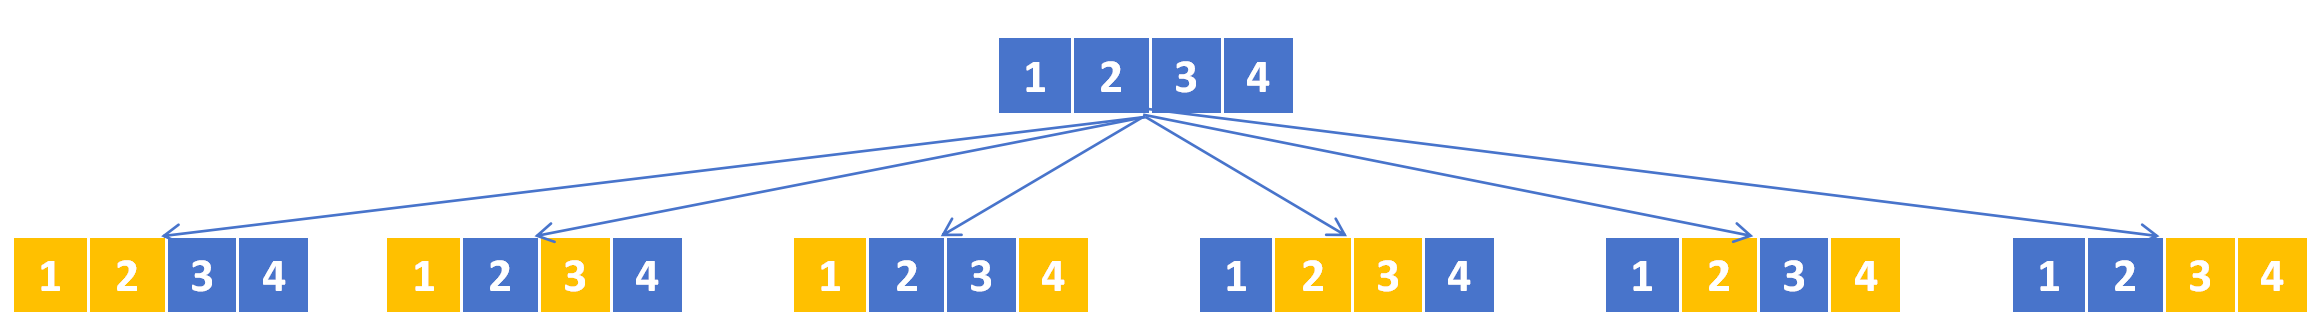
\includegraphics[width=\linewidth]{pic_resources/layer_structure.png}
	\caption{$ \binom{n}{2} $叉树层序关系}
	\label{figure1}
	\end{figure}
	
	\subsection{构造S的满射的像$ \boldsymbol{\Omega} $及其划分}
	$ \Omega $为$ S $中所有标记分量的集合。由于S中每个元素都能贡献两个标记分量，
	因此$ S $到$ \Omega $有一个满射。 \par
	
	设$ \Omega $上的一个二元关系
    $ \sim := \left\{ \left\langle a, b \right\rangle \mid a \text{与} b \text{属同一分量}, a \in \Omega, b \in \Omega \right\} $, 显然它是一个等价关系。从而$ \Omega $上有一个划分$ \sim $，它的等价类表示为:
    $ \bar{\alpha}:=\left \{ x\in\Omega \mid x\sim\bar{\alpha} \right \}  $，不妨记$ \overline{\alpha_{i}} $为第i分量的等价类，
    则$ \Omega $被$ \left \{ \overline{\alpha_{1}}, \overline{\alpha_{2}},\ldots,\overline{\alpha_{n}} \right \} $划分。
    
    \subsubsection{推论1:$ S \cong \left \{\overline{\alpha_{i}} \times \overline{\alpha_{j}} \right \}, i \neq j $}
    证明:当$ i < j $时，令\\
    \[ \sigma:S \to \left\{\overline{\alpha_{i}} \times \overline{\alpha_{j}} \right\} \]
    \[ \left(\ldots,\alpha_{i}^{\left(t_{1}\right)},\ldots,\alpha_{j}^{\left(t_{2}\right)},\ldots\right) \to \left \langle \alpha_{i}^{\left ( t_{1} \right ) } ,  \alpha_{j}^{\left ( t_{2} \right ) }\right \rangle , \left(i<j\right) 
    \]
    由S中元素的唯一性可得，当$i < j$时：
	\[
	\left(\ldots,\alpha_{i}^{\left(t_{1}\right)},\ldots,\alpha_{j}^{\left(t_{2}\right)},\ldots\right) = \left(\ldots,\left(\alpha_{i}^{\left(t_{1}\right)}\right)^{\prime},\ldots,\left(\alpha_{j}^{\left(t_{2}\right)}\right)^{\prime},\ldots\right)
	\leftrightarrow 
	\left\langle \alpha_{i}^{\left( t_{1} \right)}, \alpha_{j}^{\left( t_{2} \right) }\right\rangle =
	\left\langle \left(\alpha_{i}^{\left( t_{1} \right)}\right)^{\prime}, \left(\alpha_{j}^{\left( t_{2} \right) }\right)^{\prime}\right\rangle
	\]
	$ \sigma $是单射\\
	由$ \Omega $的定义可得，$ \sigma $是满射。\\
	综上$ \sigma $是双射，$ S \cong \left \{\overline{\alpha_{i}} \times \overline{\alpha_{j}} \right \}, i \neq j $，推论成立。

	\subsection{定义$\boldsymbol{\Omega}\times\boldsymbol{\Omega}$上的双值二元映射$f$}
	\[
	f \text{ 是映射: } \Omega \times \Omega \to \Omega \times \Omega
	\] \par
	若$ a \in \overline{\alpha_{i}^{t}}, b \in \overline{\alpha_{j}^{t}}, i \neq j $ ，则$ f\left( a,b \right) $表示将$ a,b $标记。
	由$ \overline{\alpha_{i}} $与$ \overline{\alpha_{j}} $定义以及标记的含义可知，被标记后的$ a,b $使$\left \langle a,b \right \rangle  \in \overline{\alpha_{i}} \times \overline{\alpha_{j}} $，由推论1可得$ f\left ( a,b \right )  $唯一对应$ S $的一个元素。
	
	\subsection{交互自动机的设计}
	\subsubsection{交互自动机定义}
	\begin{itemize}
		\item \textbf{有限状态集}：$ \mathbf{S} $，与3.1节$ S $的定义一致。
		\item \textbf{输入符号集}：$ \boldsymbol\Sigma = \left \{\overline{\alpha_{i}} \times \overline{\alpha_{j}} \mid i < j \right\} $，与3.2.1节讨论一致。
		\item \textbf{初始状态}：$ \boldsymbol{v} $，与3.1节$ v $的定义一致。
		\item \textbf{转移函数}：$\boldsymbol\delta(s,f(\Sigma))$，$ s \in \mathbf{S} $，$ \Sigma $为输入集，二元映射$ f $与3.3节的定义一致。它表示对于输入:
		$ \left\langle\alpha_{i}^{\tau_{i}},\alpha_{j}^{\tau_{j}}\right\rangle \in \boldsymbol\Sigma $，
		如果$ \alpha_{i}^{\tau_{i}},\alpha_{j}^{\tau_{j}} $都是$ s $中的分量，则状态转移，否则状态死亡。
		\item \textbf{终结符号集}：$ \mathbf{T} $，T取S的一个非空子集。
	\end{itemize}

	交互自动机由五元组$ \mathbf{A} = \left( \mathbf{S}, \boldsymbol\Sigma, \boldsymbol\delta, \mathbf{v}, \mathbf{T} \right) $表示。
	
	\subsubsection{交互自动机所接受的形式语言}
	引入实际交互谓词
	$ T\left(k\right)=\left\langle\alpha_{i}^{\tau_{i}\le k},\alpha_{j}^{\tau_{j}\le k}\right\rangle, \tau_{i},\tau_{j},k \in \mathbb{N} $ \par
	形如$ \prod_{k=0}^{\infty}\left ( T\left ( k \right ) \right )^{+} $的串即为该自动机所接受的形式语言，它在
	$ \binom{n}{2} $叉树上表现为一条从根节点出发到某一个子节点的路径。
	
	引入抽象交互谓词
	$ absT\left(i,j\right)=\left\langle\alpha_{i},\alpha_{j}\right\rangle $，它与实际交互谓词一一对应，将实际交互谓词替换为抽象交互谓词后，称交互自动机接受的形式语言对应的
	$ \prod_{i<j}\left(absT\left(i,j\right)\right)^{+} $为抽象交互序。
	
	\subsubsection{倾向性交互自动机}
	设映射
	$\sigma_{k}:\ \forall{x}\in\overline{\alpha_{i}},\ \sigma_{k}\left(x\right)$
	是一个$ k $元组，
	$ K_{i}=\left\{\sigma_{k}\left(x\right)\mid \forall{x} \in\overline{\alpha_{i}}\right\} $称作$ \overline{\alpha_{i}} $的特征集。\par
	若$ \Omega $中所有的等价类
	$\overline{\alpha_{1}},\overline{\alpha_{2}},\ldots,\overline{\alpha_{n}}$各具有特征集$ K_{1},K_{2},\ldots,K_{n} $，且对于任意两个$ K_{i},K_{j}$，$ \forall{x}\in{K_{i}},\forall{y}\in{K_{j}} $，$ x,y $是可比的，则称交互自动机$ \mathbf{A} = \left( \mathbf{S}, \boldsymbol\Sigma, \boldsymbol\delta, \mathbf{v}, \mathbf{T} \right) $为$ \sigma-\text{倾向性自动机} $，记作$ \boldsymbol{\sigma}-\mathbf{A} $。\par
	
	若$ \boldsymbol{\sigma}-\mathbf{A} $的输入序列可以这样被生成:\\
	设当前状态:
	\[ 
	s=
	\left( \beta _{1}^{\tau_1},\beta _{2}^{\tau_2},\ldots,\beta _{n}^{\tau_n}\right) 
	\]
	其中$ \beta _{i}^{\tau_i} \in \overline{\alpha_{i}} $，
	令$ \sigma_{k}\left(s\right)=\left( \sigma_{k}\left(\beta _{1}^{\tau_1}\right),\sigma_{k}\left(\beta _{2}^{\tau_2}\right),\ldots,\sigma_{k}\left(\beta _{n}^{\tau_n}\right)\right) $。
	
	取$g\left(\sigma_{k}\left(s\right)\right) = \left \langle \beta _{i}^{\tau_i},\beta _{j}^{\tau_j} \right \rangle $为下一个输入符号，其中$ \beta _{i}^{\tau_i},\beta _{j}^{\tau_j}$是$\left \{ \sigma \left ( \beta _{1}^{\tau_1} \right ), \sigma \left ( \beta _{2}^{\tau_2} \right ),\ldots ,\sigma \left ( \beta _{n}^{\tau_n} \right )\right \} $中符合挑选规则$ g $的两个元素的参数，交互自动机接受$ \left \langle \beta _{i}^{\tau_i},\beta _{j}^{\tau_j} \right \rangle $后进行转移并更新状态$ s $对应的分量，而转移的过程就是修改交互元具体属性的过程。
	
	\subsubsection{$ \boldsymbol{\sigma}-\mathbf{A} $的子自动机}
	\begin{itemize}
		\item 将$ \boldsymbol{\sigma}-\mathbf{A} $的初始状态$ \boldsymbol{v} $分区为两个互补子序列，沿用集合论的补集符号记这两个互补子序列分别为
		$ \boldsymbol{v^{\prime}},\complement_{v}\boldsymbol{v^{\prime}} $，使$ \boldsymbol{v} $替换为$ \boldsymbol{v^{\prime}} $。
		\item 将$ \boldsymbol{\sigma}-\mathbf{A} $的输入符号集$ \boldsymbol{\Sigma} $ 划分为两个互补集，
		$ \boldsymbol{\Sigma^{\prime}} = \left \{\overline{\alpha_{i}} \times \overline{\alpha_{j}} \mid \alpha_{i},\alpha_{j}\text{是}\boldsymbol{v^{\prime}}\text{的分量且}i < j \right\} $，补集为$ \complement_{\Sigma}\Sigma^{\prime} $，使$ \boldsymbol{\Sigma} $替换为$ \boldsymbol{\Sigma^{\prime}} $。
		\item 有限状态集$ \boldsymbol{S} $以$ \boldsymbol{v^{\prime}} $为基础构造而成。
	\end{itemize}
	作上述三处替换后的自动机为$ \boldsymbol{\sigma}-\mathbf{A} $的一个子自动机，记作$ \mathbf{sub}\left(\boldsymbol{\sigma}-\mathbf{A}\right)_{\boldsymbol{v^{\prime}}} $。

	\subsubsection{$ \mathbf{sub}\left(\boldsymbol{\sigma}-\mathbf{A}\right)_{\boldsymbol{v^{\prime}}} $的扩张}
	\begin{itemize}
		\item 	$ \forall{x} \in \complement_{v}\boldsymbol{v^{\prime}} $，使$ \boldsymbol{v^{\prime}}\cup{\left\{x\right\}}:= \boldsymbol{v^{\prime\prime}},\ \complement_{v}\boldsymbol{v^{\prime}}\setminus{\left\{x\right\}}:=\complement_{v}\boldsymbol{v^{\prime\prime }} $。
		\item 将$ \boldsymbol{\sigma}-\mathbf{A} $的输入符号集$ \boldsymbol{\Sigma} $ 划分为两个互补集，
		$ \boldsymbol{\Sigma^{\prime\prime}} = \left \{\overline{\alpha_{i}} \times \overline{\alpha_{j}} \mid \alpha_{i},\alpha_{j}\text{是}\boldsymbol{v^{\prime\prime}}\text{的分量且}i < j \right\} $，补集为$ \complement_{\boldsymbol{\Sigma}}\boldsymbol{\Sigma^{\prime\prime}} $，使$ \boldsymbol{\Sigma} $替换为$ \boldsymbol{\Sigma^{\prime\prime}} $。
		\item 有限状态集$ \boldsymbol{S} $以$ \boldsymbol{v^{\prime\prime}} $为基础构造而成。
	\end{itemize}
	作上述三处替换后的自动机为$ \mathbf{sub}\left(\boldsymbol{\sigma}-\mathbf{A}\right)_{\boldsymbol{v^{\prime}}} $的一个扩张，由于仍为子自动机，不妨记作$\mathbf{sub}\left(\boldsymbol{\sigma}-\mathbf{A}\right)_{\boldsymbol{v^{\prime\prime}}} $。
	
	\subsubsection{正规子自动机}
	若$ \forall{m}>0 $，$ \mathbf{sub}\left(\boldsymbol{\sigma}-\mathbf{A}\right)_{\boldsymbol{v}} $产出$ m $长度的抽象交互序$ q $，$ \exists{n}>0, n<m $，使得$ \mathbf{sub}\left(\boldsymbol{\sigma}-\mathbf{A}\right)_{\boldsymbol{v^{\prime}}} $产出$ n $长度的抽象交互序$ p $是$ q $的子序列，则称$ \mathbf{sub}\left(\boldsymbol{\sigma}-\mathbf{A}\right)_{\boldsymbol{v}} $正规于$ \mathbf{sub}\left(\boldsymbol{\sigma}-\mathbf{A}\right)_{\boldsymbol{v^{\prime}}} $，记作$ \mathbf{sub}\left(\boldsymbol{\sigma}-\mathbf{A}\right)_{\boldsymbol{v}}\trianglelefteq \mathbf{sub}\left(\boldsymbol{\sigma}-\mathbf{A}\right)_{\boldsymbol{v^{\prime}}}$。\par
	需要注意的是，$ A $扩张后的$ A_{x} $仍有可能使$ A_{x} \trianglelefteq A $。\par
	为简便表示，若$ A $表示为子自动机，则$ A_{x} $表示$ A $加入了$ x $进行扩张的新子自动机；$ A^{\left(i\right)} $表示，$ A $加入了$ i $个元素后的一个扩张。
	正规子自动机有如下性质：\\
	\textbf{以下性质使用统一假设：$ A,A_{x},A_{y},A_{z},A_{x,y},A_{x,z},A_{y,z} $产出的非空抽象交互序分别为$ q_{0},q_{1},q_{1}^{\prime},q_{1}^{\prime\prime},q_{2},q_{2}^{\prime},q_{2}^{\prime\prime} $，这四个自动机按握手定理共有6条连线，而每条连线可以分配$\left\{\text{连接},\text{不连接}\right\}\times\left\{\text{正向},\text{反向}\right\}$四种属性，其中把不连接的归为同一类，则共有$ 3^{6} $种连接属性，这里只研究与本文主题相关的部分。}。
	\begin{enumerate}
		\item \textbf{传递性}：若$ A \trianglelefteq B, B \trianglelefteq C $，则$ A \trianglelefteq C $。\\证：设$ A,B,C $分别产出的抽象交互序$ q_{1},q_{2},q_{3} $，由条件可知$ q_{1} $是$ q_{2} $的子序列，$ q_{2} $是$ q_{3} $的子序列，显然$ q_{1} $是$ q_{3} $的子序列，由正规子自动机定义可得：$ A \trianglelefteq C $。
		\item \textbf{可易性}：$ A_{xy}=A_{yx} $\\证：显然因为它们是同一个子自动机。
		\item \textbf{性质1}：$ A_{x} \trianglelefteq A_{y} \Rightarrow A_{x} \trianglelefteq A $\\证：如果$ q_{1} $包含$ x $的符号，那么它一定不是$ q_{1}^{\prime} $的子序列，这是矛盾的，则$ q_{1} $只能是$ q_{0} $的子序列，从而$ A_{x} \trianglelefteq A $。
		\item \textbf{性质2}：$ A \trianglelefteq A_{x} \trianglelefteq A_{y} \Leftrightarrow q_{0}=q_{1} $\\证：由性质一，$ A \trianglelefteq A_{x} \trianglelefteq A_{y} \Leftrightarrow A \trianglelefteq A_{x} \wedge A_{x} \trianglelefteq A \Leftrightarrow q_{0}=q_{1} $。
		\item \textbf{性质3}：$ A_{x} \trianglelefteq A_{y} \wedge A \trianglelefteq A_{x,y} \Rightarrow A_{x} \trianglelefteq A_{x,y} $\\证：由性质一和传递性，$ A_{x} \trianglelefteq A_{y} \wedge A \trianglelefteq A_{x,y} \Rightarrow A_{x} \trianglelefteq A \trianglelefteq A_{x,y} \Rightarrow A_{x} \trianglelefteq A_{x,y} $。
	\end{enumerate}
	
	\subsection{$ \boldsymbol{\sigma}-\mathbf{A} $生成的输入序列的封闭性}
	若$ \boldsymbol{\sigma}-\mathbf{A} $具备3.4.3节所描述的自举能力，则$ \boldsymbol{\sigma}-\mathbf{A} $生成的每个输入符号封闭到它的输入符号集$ \boldsymbol{\Sigma} $，定义为封闭性。
	
	\subsection{$ \boldsymbol{\sigma}-\mathbf{A} $生成的输入序列的一致性}
	定义$ \boldsymbol{\sigma}-\mathbf{A} $生成的输入序列的一致性为：设当前$ \boldsymbol{\sigma}-\mathbf{A} $处于任意可转移状态$ s $，$ \forall{n}\in\mathbb{N},n>0 $，$ \boldsymbol{\sigma}-\mathbf{A} $执行了n次交互，产生了$ n $长度的输入序列$ q $。若令$ \boldsymbol{\sigma}-\mathbf{A} $从状态$ s $出发重复上述操作任意次，得到的$ n $长度$ q $都是一致的，则称$ \boldsymbol{\sigma}-\mathbf{A} $是一致的。\par
	设$ \omega=\left\{ w_{1},w_{2},\ldots,w_{n}\right\} $是当前抽象交互序列$ q $中相同但位置不同的的连续子序列的集合，记$ w_{i}\rightarrow x_{i}$表示$ x_{i} $是$ w_{i} $在$ q $中的后继，记$ prev\left(w_{i}\right) $为$ w_{i} $在$ q $中的前驱。记
	$ \mathbb{X}=\left\{ x_{1},x_{2},\ldots,x_{n} \right\} $为$ \omega $所有元素的后继的集合。\par
	观察到对任一$ w_{i} $加入它的前驱，使$ w_{i}=w_{i}+prev\left(w_{i}\right) $，仍有
	$ w_{i}\rightarrow x_{i} $，由于$ \forall w_{i} \in \omega $也有$ w_{i} \in q $，不断地使$ w_{i}=w_{i}+prev\left(w_{i}\right) $，最终每一个$ w_{i} $都将是由$ q $的首符号$ q_{0} $出发构造而成的子序列。\par
	
	对$ \omega $作一个划分：$ w_{i}\sim w_{j}\Leftrightarrow\left\{w_{i},w_{j}\in \omega \mid w_{i}\rightarrow x\wedge w_{j}\rightarrow x\right\} $，将$ \omega $按等价类划分为
	$ \omega^{\prime}=\left\{\overline{w_{1}},\overline{w_{2}},\ldots\right\} $，则存在一个映射$ \zeta:\omega^{\prime}\rightarrow\mathbb{X} $，$ \zeta $是一个双射。\par
	
	$ \forall{\overline{w_{i}}} \in \omega^{\prime} $，构造对应的输入序列并输入到$ \boldsymbol{\sigma}-\mathbf{A} $，若$ \boldsymbol{\sigma}-\mathbf{A} $的输出的下一个输入符号为$ \zeta\left(\overline{w_{i}}\right) $，则称$ \overline{w_{i}} $为稳定连续子序列。
	
	\subsection{$ \boldsymbol{\sigma}-\mathbf{A} $生成的输入序列的有效性}
	定义$ \binom{n}{2} $叉树的\textbf{位置占比}为一个节点到其所在层的最左兄弟节点的距离与该层总节点数之比。\par
	根据3.1.1节描述的$ \binom{n}{2} $叉树的格局布置，若$ \boldsymbol{\sigma}-\mathbf{A} $生成的每一个输入符号的位置占比所形成的数列是有界的，则称该生成的输入序列是有效的。\par
	假设当前第$ t $次交互后状态为
	\[
	s=\left(\eta_{1},\eta_{2},\ldots,\eta_{n}\right)
	\]
	若执行转移$\boldsymbol\delta(s,f(\left\langle \eta_{i},\eta_{j} \right\rangle ))$，其中$ j>i $，则根据格局布置，转移后的状态节点$ s^{\prime} $位置相对于其父节点的最左子节点为
	$ p\left(i,j\right)=\frac{\left(2n-i\right)\left( i-1 \right)}{2}+\left(j-i \right) $。假设$ s^{\prime} $的父节点的位置相对于其所在层最左的兄弟节点为$ fp $，那么可以得到$ s^{\prime} $的绝对位置
	\[ p_{d}\left(i,j\right) =\left(p_{f}-1\right)\binom{n}{2}+p\left(i,j\right) \]
	初始化$ p_{f}=1 $，每次交互结束后，令$ p_{f}=p_{d}\left(i,j\right) $，从而递归地得到抽象交互序中每一个符号对应地节点在其所处层的相对于最左兄弟节点的位置。\par
	综上递归地定义抽象交互序的上分位占比为
	\[ r\left(t\right)=\frac{p_{d}\left(i,j\right)}{\binom{n}{2}^{t}} \]
	其中$ i<j,t\text{表示第t次交互} $。\par
	由$ \mathbf{R_{p}}=\left\{r\left(1\right),r\left(2\right),\ldots,r\left(k\right)\right\} $作为线性回归分析的材料，预测$ r\left(k+1\right) $，若$ r\left(k+1\right) $的残差小于某个$ \epsilon>0 $，则认为当前抽象交互序是有效的，显然这是一个后验的结论，该性质需要迭代模型进行数据采集后才能确定。

	\section{完备$ \boldsymbol{\sigma}-\mathbf{A} $}
	当$ \boldsymbol{\sigma}-\mathbf{A} $具备封闭性和一致性时，称$ \boldsymbol{\sigma}-\mathbf{A} $为完备的，记作
	$ \boldsymbol{Com}\left(\sigma-A\right) $。\\
	\textbf{命题4}：$ \boldsymbol{Com}\left(\sigma-A\right) $的正规子自动机$ \boldsymbol{sub}\left(Com\left(\sigma-A\right)\right) $也是完备的，证：
	\begin{itemize}
		\item \textbf{封闭性}：由于正规子自动机仍是倾向性自动机，所以继承封闭性。
		\item \textbf{一致性}：设
		$ 
		\boldsymbol{Com}\left(\sigma-A\right),
		\boldsymbol{sub}\left(Com\left(\sigma-A\right)\right) 
		$
		分别产出的抽象交互序为$ q_{0},q_{1} $，由正规性得$ q_{1} $ 是 $ q_{0} $的子序列，$ q_{0} $的出现蕴含着$ q_{1} $的出现，从而
		$ \boldsymbol{Com}\left(\sigma-A\right) $的一致性蕴含着
		$ \boldsymbol{sub}\left(Com\left(\sigma-A\right)\right) $的一致性。
	\end{itemize}
	综上若
	$ 
	\boldsymbol{sub}\left(Com\left(\sigma-A\right)\right) 
	\trianglelefteq 
	\boldsymbol{Com}\left(\sigma-A\right)
	$，
	则$ \boldsymbol{sub}\left(Com\left(\sigma-A\right)\right) $也是完备的。
	
	\subsection{循环$ \boldsymbol{Com}\left(\sigma-A\right) $}
	设$ \boldsymbol{Com}\left(\sigma-A\right) $的抽象交互序$ q $，$ q^{\prime} $是$ q $的连续子序列，$ \left\langle q^{\prime} \right\rangle = \left(q^{\prime}\right)^{*}w,\ w\text{是}q^{\prime}\text{的前缀且可为空} $。若$ q=\left\langle q^{\prime} \right\rangle $，则称$ \boldsymbol{Com}\left(\sigma-A\right) $是循环的，$ q^{\prime} $是$ q $的生成元。
	
	\subsubsection{循环$ \boldsymbol{Com}\left(\sigma-A\right) $的正规子自动机}
	所有正规于循环$ \boldsymbol{Com}\left(\sigma-A\right) $的子自动机也是循环的，证：\\
	设
	$ 
	\boldsymbol{sub}\left(Com\left(\sigma-A\right)\right) 
	\trianglelefteq 
	\boldsymbol{Com}\left(\sigma-A\right)
	$，
	且$ 
	\boldsymbol{Com}\left(\sigma-A\right),
	\boldsymbol{sub}\left(Com\left(\sigma-A\right)\right) 
	$
	分别产出的抽象交互序为$ q_{0},q_{1} $，其中$ \mu $是$ q_{0} $的生成元，
	由第4节命题4知$ \boldsymbol{sub}\left(Com\left(\sigma-A\right)\right) $是完备的。不妨取$ \mu $与$ q_{1} $的公共子序列$ \lambda $，则$ \lambda $是$ q_{0} $中子序列$ q_{1} $的生成元，从而$ \left\langle \lambda \right\rangle = q_{1} $，
	从而$ \boldsymbol{sub}\left(Com\left(\sigma-A\right)\right) $也是循环的。
	
	\subsubsection{循环$ \boldsymbol{Com}\left(\sigma-A\right) $的正规充要条件}
	设$ A,B $是生成元分别为$ a,b $的循环$ \boldsymbol{Com}\left(\sigma-A\right) $，证明：
	\[A \trianglelefteq B \Leftrightarrow a\text{是}\left\langle b \right\rangle \text{的子序列}\]
	充分性：若$ a\text{是}\left\langle b \right\rangle \text{的子序列} $，则存在$ t $个$ b $组成的序列$ bb\ldots b $，使$ a $是$ bb\ldots b $的子序列，从而$ \left\langle a \right\rangle $是$ \left\langle bb\ldots b \right\rangle = \left\langle b \right\rangle $的子序列，从而$ A \trianglelefteq B $。\\
	必要性：若$ A \trianglelefteq B $，则存在$ t $个$ b $组成的序列$ bb\ldots b $，使$ a $是$ bb\ldots b $的子序列，从而$ \left\langle a \right\rangle $是$ \left\langle bb\ldots b \right\rangle = \left\langle b \right\rangle $的子序列。
	
	\subsection{正规的种类}
	设$ A \trianglelefteq B$，$ a,b $分别是$ A,B $生成的抽象交互序，研究$ a $与$ b $在结构上的各种联系，用诸不同的联系为正规分类，它们都具备正规的\ \ 条性质，遂不再赘述。
	
	\subsubsection{后缀正规}
	假设$ A \trianglelefteq A_{x} $，且$ A,A_{x} $分别产出不为空的抽象交互序$q^{\prime},q$。
	当$ q^{\prime} $是$ q $的后缀连续子序列，称这种正规形式为后缀正规，记$ A\ bwk\ A_{x} $，非前缀正规记作$ A\ nbwk\ A_{x} $。\par
	\textbf{右移作用}：后缀正规也可以看作是将子自动机生成的输入序列在其后缀正规的扩张自动机生成的输入序列上执行右移，记$ bwk_{t} $为右移$ t $个位置。
	
	\subsubsection{反转正规}
	假设$ A,A_{x} $都是循环$ \boldsymbol{Com}\left(\sigma-A\right) $，且$q^{\prime},q$分别是它们的生成元。
	记$ \overline{str} $是将$ str $这个串左右翻转后的串，当$ \left\langle \overline{q^{\prime}} \right\rangle $是
	$ \left\langle q \right\rangle $的子序列，称这种正规形式为反转正规，记为$ A\ rvs\ A_{x} $，非反转正规记作$ A\ nrvs\ A_{x} $。\par
	\textbf{引理1}\ \ 若$ \left\langle \overline{a} \right\rangle $是$ \left\langle b \right\rangle $的子序列，则$ \left\langle a \right\rangle $是$ \left\langle \overline{b} \right\rangle $的子序列，证：\par
	$ \overline{a} $是若干个$ b $组成的序列$ bb\ldots b $的子序列，则$ a $是$ \overline{bb\ldots b} $的子序列，又$ \overline{bb\ldots b} = \overline{b}\ \overline{b}\ldots\overline{b} $，从而$ \left\langle a \right\rangle $ 是 $ \left\langle \overline{b}\ \overline{b}\ldots\overline{b} \right\rangle = \left\langle \overline{b} \right\rangle $的子序列。\par
	\textbf{性质1}\ \ 若$ A\ rvs\ A_{x}\ rvs\ A_{x,y} $，则$ A \trianglelefteq A_{x,y} $，证：\par
	假设$ q^{\prime\prime},q^{\prime},q $分别是$ A,A_{x},A_{x,y} $的生成元。$ \left(A\ rvs\ A_{x}\right) \rightarrow \left\langle \overline{q^{\prime\prime}} \right\rangle $是$ \left\langle q^{\prime} \right\rangle $的子序列，$ \left(A_{x}\ rvs\ A_{x,y}\right) \rightarrow \left\langle \overline{q^{\prime}} \right\rangle $是$ \left\langle q \right\rangle $的子序列，由引理1得$ \left\langle q^{\prime\prime} \right\rangle $是$ \left\langle \overline{q^{\prime}} \right\rangle $的子序列，从而$ \left\langle q^{\prime\prime} \right\rangle $是$ \left\langle q \right\rangle $的子序列，得$ A \trianglelefteq A_{x,y} $。\par
	\textbf{推论1}\ \ 推广性质1到规模为$ t $个元素的扩张：若$ A\ rvs\ A_{1}\ rvs\ \ldots\ rvs\ A_{1,2,\ldots,t} $，则$ A \trianglelefteq \ldots \trianglelefteq A_{2k} $且$ A_{1} \trianglelefteq \ldots \trianglelefteq A_{2k+1} $，证：\\
	对相邻三个$ A_{i}\ rvs\ A_{i+1}\ rvs\ A_{i+2},\ 1 \le i \le t-2 $，使用性质1，再使用正规的传递性即可得证。\par
	
	\subsubsection{轮换正规}
	假设$ A $的生成元$ q^{\prime\prime}=\left(x_{1},x_{2},\ldots,x_{n}\right) $，则$ \left(x_{n},x_{1},\ldots,x_{n-1}\right) $为$ q^{\prime\prime} $的一次右轮换，记为$ \overset{q^{\prime\prime}}{\rightarrow} $。假设$ A_{x} $的生成元是$ q $，若$ \left\langle\overset{q^{\prime\prime}}{\rightarrow}\right\rangle $是$ \left\langle q \right\rangle $的后缀连续子序列，则称$ A $右轮换正规于$ A_{x} $，记为$ A\ rloop\ A_{x} $。同理可以定义左轮换正规：若$ \left\langle \overset{q^{\prime\prime}}{\leftarrow} \right\rangle $是$ \left\langle q \right\rangle $的后缀连续子序列，则称$ A $左轮换正规于$ A_{x} $，记为$ A\ lloop\ A_{x} $。与3.5.2右移作用同理，记$ rloop_{t} $用于描述$ \overset{q^{\prime\prime}}{\rightarrow} $向右移动了t个位置。\par
	\textbf{性质1}\ \ 已知$ q={x_{1}x_{2}\ldots x_{k}} $是$ A_{1} $的生成元，若$ A_{1}\ rloop_{i}\ \ldots\ rloop_{i}\ A_{k+1} $，则$ A_{1} \trianglelefteq A_{k+1}$，$ i $为任意非负整数。
	
	\subsection{正规网络}
	本节提出一个如图2所示的网络结构，它旨在研究$ \boldsymbol{\sigma}-\mathbf{A} $从初始规模$ A $出发，在不同扩张情况下，某些行为的持续与被正规性质保持的抽象交互序的上下文关系是否高度相关：比如$ A $表现的行为是绕形心右旋$ \frac{\pi}{2} $后，扩张为了$ A_{x} $它绕形心右旋$ \frac{\pi}{2} $后向右下方平移一个单位，如果$ A \trianglelefteq A_{x} $，那么可定性$ A $的抽象交互序与绕形心右旋$ \frac{\pi}{2} $行为是相关的。\par
	图2所示网络从左到右分为$ k+1 $层，第$ i $层有$ \binom{k+1}{i} $个，它表示第i层都是加入了$ i $个不同交互元的扩张。本节给出一般的分类方法：
	\begin{enumerate}
		\item \textbf{层内分类}：对于同一层的所有扩张，依据正规的传递性，以处于同一正规链为等价关系划分该层。再依据正规的性质1和2，假设$ A_{x} \trianglelefteq A_{y} \trianglelefteq A_{z} $，若$ A \trianglelefteq A_{y} $，则$ q_{0}=q_{1}^{\prime}=q_{1}^{\prime\prime} $，$ q_{1} $是$ q_{0} $的子序列。
		\item \textbf{层间分类}：假设已经执行了层内分类，再依据性质3对于不同层进一步分类：假设$ A_{x} \trianglelefteq A_{y} \trianglelefteq A_{z} $，此时只需要考察$ A $对所有二阶扩张$ \left\{A_{x,y},A_{x,z},A_{y,z}\right\} $的正规性，若$ A \trianglelefteq A_{x,y} $，则$ A_{x} \trianglelefteq A_{x,y} $，从而建立一阶扩张层和二阶扩张层的联系。
	\end{enumerate}
	\begin{figure}[H]
		\centering
		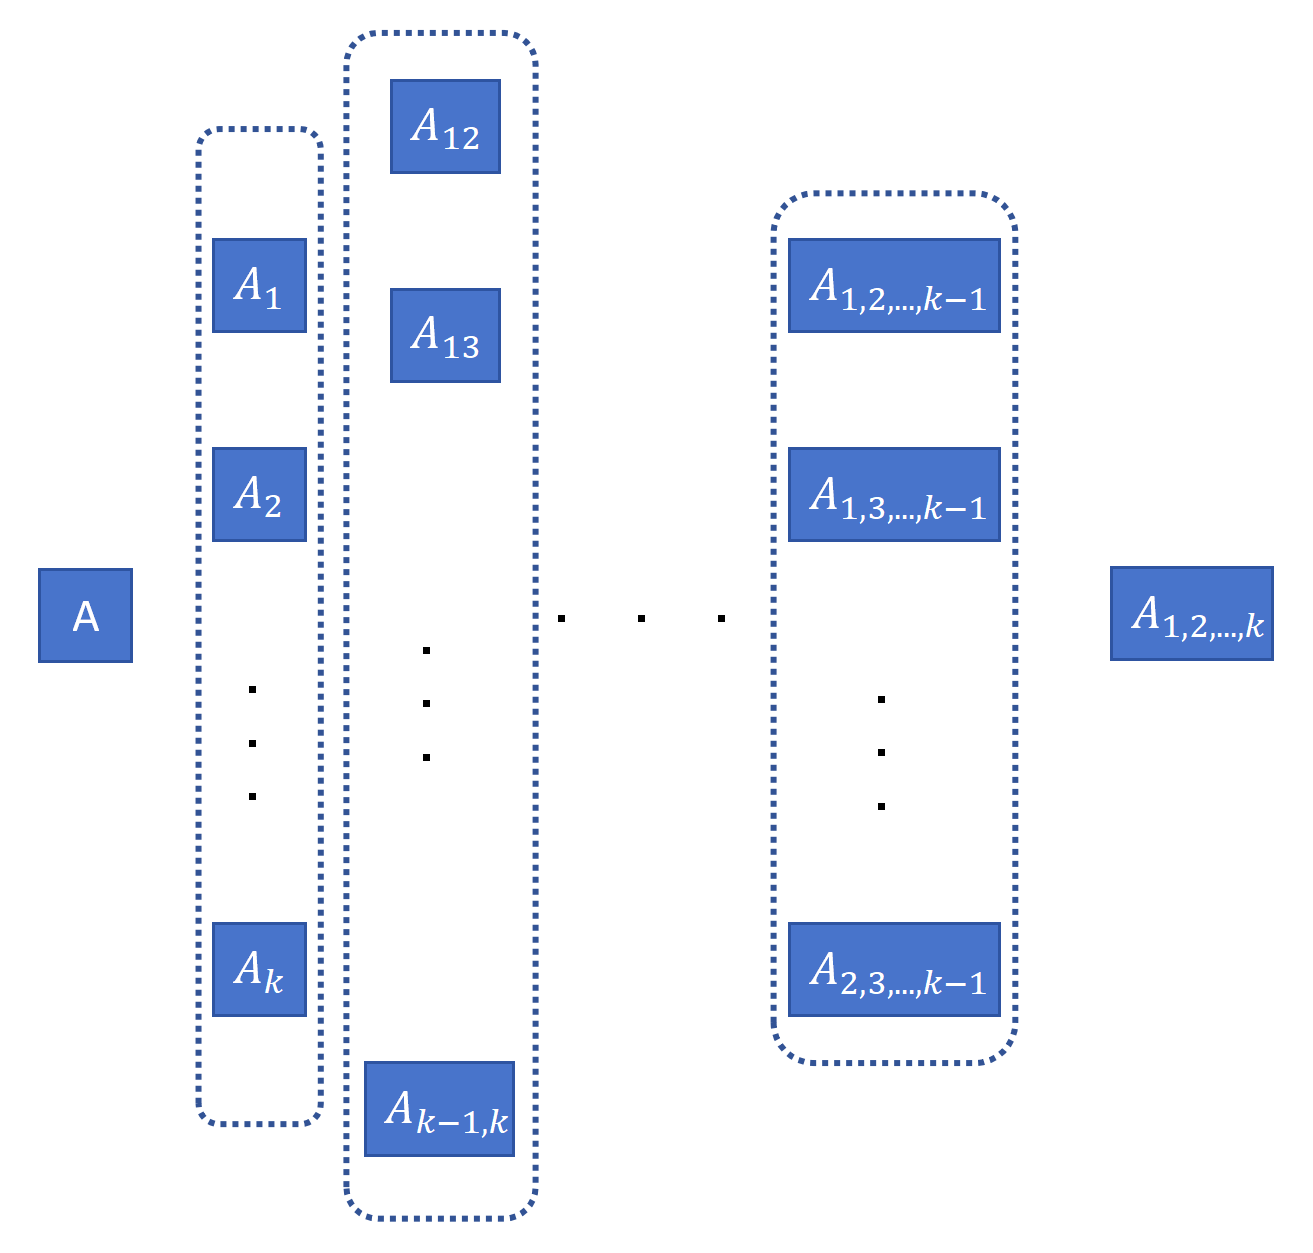
\includegraphics[width=0.7\linewidth]{pic_resources/formalization_structure.png}
		\caption{正规网络架构}
		\label{figure2}
	\end{figure}
	
	\section{生命游戏模型}
	\subsection{生命游戏简述}
	\begin{enumerate}
		\item \textbf{网格}：游戏在一个二维的网格上进行，每个格子可以是“活”或“死”状态。
		\item \textbf{初始状态}：游戏从一个初始状态开始，玩家可以任意设置哪些格子是活的，哪些是死的。
		\item \textbf{邻居}：每个格子有八个邻居，即上下左右和对角线方向的格子。
		\item \textbf{规则}：
		\begin{itemize}
			\item \textbf{存活}：一个活的格子如果有2或3个活的邻居，它会继续存活。
			\item \textbf{死亡}：一个活的格子如果有少于2个或多于3个活的邻居，它会死亡（孤独或过度拥挤）。
			\item \textbf{繁殖}：一个死的格子如果有正好3个活的邻居，它会变成活的。
		\end{itemize}
	\end{enumerate}
	\subsection{生命游戏模型转化为$ \boldsymbol{\sigma}-\mathbf{A} $}
	通过以下构造方法，可以把生命游戏模型的一次迭代等价为多个交互的复合，从而将生命游戏模型转化为$ \boldsymbol{\sigma}-\mathbf{A} $。
	\begin{enumerate}
		\item \textbf{交互元}：取包含模型的所有活格子及其邻居格子作为交互元集。每个交互元维护
		\begin{itemize}
			\item \textbf{$ buffer_{0} $}： 记录交互过的死格子个数
			\item \textbf{$ buffer_{1} $}： 记录交互过的活格子个数
			\item \textbf{$ buffer_{2} $}： 记录交互过的格子编码
			\item \textbf{$ sign $}： 表示自身是否可交互
			\item \textbf{$ result $}:存储状态转移的结果。
		\end{itemize}
		\item \textbf{扩张}：当增加交互元时，保持原交互元的编号，新增的交互元从上到下，从左到右延续编号。
		\item \textbf{收缩}：当减少交互元时，保持现有交互元的编号。
		\item \textbf{特征提取函数}：从上到下，从左到右为交互元从1开始编号。
		\item \textbf{挑选规则}：取当前编号最小和次小且各自的$ buffer_{2} $中没有记录对方的两个可交互的交互元。
		\item \textbf{交互元状态转移}：
		\begin{itemize}
			\item \textbf{$ buffer_{1}>3 $}:$ result $置为死亡状态，且$ sign $置$ false $表示不可交互。
			\item \textbf{$ buffer_{0}>6 $}：$ result $置为死亡状态，且$ sign $置$ false $表示不可交互。
			\item \textbf{$ buffer_{0}=3且buffer_{1}=5 $}：$ result $置为存活状态。
			\item \textbf{其他情况}：格子状态不变。
		\end{itemize}
		\item \textbf{交互结束}：当所有交互结束后，各格子将状态更新为$ result $。
	\end{enumerate}

	\subsubsection{转化的$ \boldsymbol{\sigma}-\mathbf{A} $具有完备性}
	显然，通过上述方法将生命游戏模型转化为$ \boldsymbol{\sigma}-\mathbf{A} $的是完备的：
	一次迭代转化为多次交互的复合，使封闭性满足；生命游戏的规则一致性蕴含了$ \boldsymbol{\sigma}-\mathbf{A} $的一致性。
	\subsubsection{转化程序设计}
	图3表示接受一个具体模型，并转化为对应的$ \boldsymbol{Com}\left(\sigma-A\right) $的程序设计，程序可以在GitHub中获取：\href{https://github.com/Nomel-Cool/IA.git}{$ \boldsymbol{Com}\left(\sigma-A\right) $转化程序}。
		\begin{figure}[H]
		\centering
		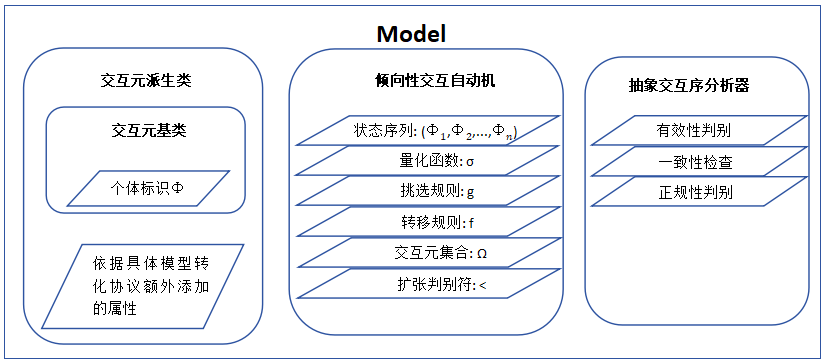
\includegraphics[width=\linewidth]{pic_resources/new_program_class.png}
		\caption{转化程序类设计图}
		\label{figure4}
	\end{figure}
	\begin{enumerate}
		\item 首先需要继承交互元基类，依赖4.2节的转化规则添加$ buffer_{0},buffer_{1},buffer_{2},sign,result $字段。
		\item 然后将模型转化为对应的交互元序列表示其状态序列，依次实现量化函数，挑选规则，转移规则，交互元集合以及扩张判断（利用交互元集合是否被包含来判断另一个倾向性交互自动机是否为自身的扩张）
		\item 将每次实际交互有序对抽象为抽象交互有序对并传输到抽象交互序分析器，它用于建立抽象交互序，提供2.4.6节提到的正规性检查，2.6节提到的一致性检查以及2.7节提到的有效性判别。
	\end{enumerate}
	\subsection{滑翔机模型与循环$ \boldsymbol{Com}\left(\sigma-A\right) $}
	如图$ \left(a\right) $到图$ \left(d\right) $所示的四个
	$ 3 \times 3 $点阵是滑翔机模型的4种迭代：
	\[ \left(glider_{1}, glider_{2}, glider_{3}, glider_{4}\right) \]构成一个$ 4-\text{轮换} $。\par
	假设$ glider $轮换过程中产出的抽象交互序为$ q $，其中$ glider_{i}\rightarrow glider_{\left(i+1\right) \bmod 4} $产出抽象交互序$ q_{i} $，由4.2.2节保证了其不变性。显然$ q_{1}q_{2}q_{3}q_{4} $是$ q $的一个生成元，由4.2.1节知$ glider $转化的$ \boldsymbol{\sigma}-\mathbf{A} $是完备的，上述可得$ \boldsymbol{Com}\left(\sigma-A\right) $是循环的。
	\begin{figure}[h]  
		\centering  
		\begin{subfigure}[b]{0.12\textwidth}  
			\centering  
			
\includegraphics[width=\textwidth]{pic_resources/glider1.png}
			\caption{$glider_{1}$}  
		\end{subfigure}  
		\hfill % 添加一些水平间距  
		\begin{subfigure}[b]{0.12\textwidth}  
			\centering  
			
\includegraphics[width=\textwidth]{pic_resources/glider2.png}
			\caption{$glider_{2}$}  
		\end{subfigure}  
		\hfill % 添加一些水平间距  
		\begin{subfigure}[b]{0.12\textwidth}  
			\centering  
			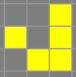
\includegraphics[width=\textwidth]{pic_resources/glider3.png}
			\caption{$glider_{3}$}  
		\end{subfigure}  
		\hfill % 添加一些水平间距  
		\begin{subfigure}[b]{0.12\textwidth}  
			\centering  
			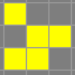
\includegraphics[width=\textwidth]{pic_resources/glider4.png}
			\caption{$glider_{4}$}  
		\end{subfigure}  
		\caption{Glider examples}  
	\end{figure}  
	\subsection{滑翔机发射器模型与循环$ \boldsymbol{Com}\left(\sigma-A\right) $}
	图5为滑翔机发射器Gosper glider gun的初始模式。由于生成glider时没有改变其bound box，于是利用python脚本可以对同一范围检测矩阵迭代周期，结果为60，同理假设$ 60-\text{轮换} $过程产出$ q_{1},q_{2},\ldots,q_{60} $，则Gosper glider gun对应的循环$ \boldsymbol{Com}\left(\sigma-A\right) $的生成元就是
	$ q_{1}q_{2}\ldots q_{60} $。\par
	上述python脚本可以访问GitHub链接获取：
	\href{https://github.com/Nomel-Cool/DetectSteadyModelPeriod.git}{Life Game模型周期检测脚本文件}
	\begin{figure}[H]
		\centering
		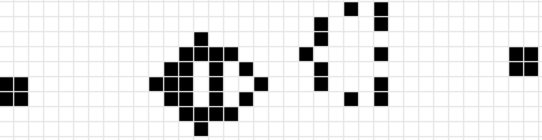
\includegraphics[width=0.5\linewidth]{pic_resources/gosper_glider_gun.png}
		\caption{$ Gosper\ glider\ gun $}
		\label{figure3}
	\end{figure}

	\subsection{glider的扩张与glider gun}
	显然4.3节描述的glider对应的$ \boldsymbol{Com}\left(\sigma-A\right)_{\text{glider}} $是正规于4.4节描述的Gosper glider gun对应的$ \boldsymbol{Com}\left(\sigma-A\right)_{\text{gun}} $循环子自动机。
	利用4.2.2节的转化程序提供的正规性检查，可以轻松得到上述结论。由此可以仅通过$ \boldsymbol{Com}\left(\sigma-A\right)_{\text{glider}} $生成的串是否正规于某个$ \boldsymbol{Com}\left(\sigma-A\right) $，就可以代替视觉的上判断$ \boldsymbol{Com}\left(\sigma-A\right) $是否生成glider。
	
	\newpage
	\section{结论}
	\subsection{工作结果}
	\begin{enumerate}
		\item 定义了倾向性交互自动机
		\item 定义了倾向性交互自动机的正规性
		\item 研究了正规性的若干性质
		\item 定义了正规网络，并给出了正规网络的分类方法
		\item 构造了一种转化方法，使生命游戏模型转化为一个倾向性交互自动机
		\item glider和glider gun两种bound box不变的生命游戏模型与循环倾向性交互自动机是等价的
		\item 未完待续
	\end{enumerate}
	
	\subsection{研究方向}
	\begin{enumerate}
		\item 为正规分类的工作并不完全，找到串与其子串的所有结合模式，一个模式一一对应一种正规类型。
		\item 利用现有的$ \boldsymbol{\sigma}-\mathbf{A} $形态和正规分类，描述元胞自动机的所有基础模式分类。
	\end{enumerate}
	
	\phantomsection\addcontentsline{toc}{section}{参考文献}\tolerance=500
	\renewcommand{\refname}{参考文献}
	\begin{thebibliography}{99}
		\bibitem{wolfram2002new} Wolfram, Stephen. \textit{A New Kind of Science}. Wolfram Media, 2002.
		\bibitem{rotman2010advanced} Rotman, Joseph J. \textit{Advanced Modern Algebra}. American Mathematical Society, 2010.
	\end{thebibliography}

\end{document}